\documentclass[a4paper,12pt,twoside]{scrreprt}
% Autor der Vorlage: Klaus Rheinberger, FH Vorarlberg
% 2017-02-20

%% Hilfe: z.B.
% empfohlener Einstieg: http://latex.tugraz.at/  
% https://de.wikibooks.org/wiki/LaTeX-Kompendium:_Schnellkurs:_Erste_Schritte
% https://de.wikibooks.org/wiki/LaTeX-Kompendium:_Schnellkurs
% https://de.wikibooks.org/wiki/LaTeX-Kompendium

%% Pakete:
% Der Befehl \usepackage[latin9]{inputenc} ermöglicht die direkte Angabe von Umlauten. Übrigens lässt sich so auch das Euro-Zeichen direkt eingeben. Auf Betriebssystemen, wie zum Beispiel allen neueren Linux-Distributionen, verwendet man statt \usepackage[latin9]{inputenc} besser \usepackage[utf8]{inputenc}, auf Applesystemen verwendet man \usepackage[macce]{inputenc} (oder das für ältere Modelle gültige \usepackage[applemac]{inputenc}).
\usepackage[utf8]{inputenc}
\usepackage[T1]{fontenc}    % Silbentrennung bei Sonderzeichen
\usepackage{graphicx}       % Bilder einbinden
\usepackage[ngerman]{babel} % Deutsche Sprachanpassungen
\usepackage{csquotes}       % When using babel or polyglossia with biblatex, loading csquotes is recommended to ensure that quoted texts are typeset according to the rules of your main language.
\usepackage{acronym}  % für optionales Abkürzungsverzeichnis
\usepackage{eurosym}  % z. B. \EUR{12345,68}
\usepackage[linktocpage=true]{hyperref} % Links z. B. \href{https://www.wikibooks.org}{Wikibooks home}
\usepackage[bindingoffset=8mm]{geometry}% Bindeverlust von 8mm einbeziehen. Mit dem geometry-Paket können Sie die Ränder auch ganz individuell anpassen.
\usepackage{caption} % Abbildungslegenden
\captionsetup{format=hang, justification=raggedright}
\usepackage{pdfpages} %um PDFs im Anhang zu inkludieren
\usepackage{fancyhdr}
\usepackage{longtable}
\usepackage[]{algorithm2e}
\usepackage{float}
\usepackage{makecell}

\usepackage{pgf,tikz,pgfplots}
\usepackage{amsmath}
\pgfplotsset{compat=1.15}
\usepackage{mathrsfs}
\usetikzlibrary{arrows}
\pagestyle{empty}

\pagestyle{fancy}
\renewcommand{\headrulewidth}{0.4pt}
\renewcommand{\footrulewidth}{0.4pt}
\fancyhf{} % clear all fields
\fancyhead[R]{Emrah Öztürk, Michael Schneider, Nicolai Schwartze}
%\fancyfoot[C]{\thepage}
\fancypagestyle{plain}{%
	\renewcommand{\headrulewidth}{0.4pt}%
	\renewcommand{\footrulewidth}{0.4pt}%
	\fancyhf{}% clear all fields
	\fancyhead[R]{Emrah Öztürk, Michael Schneider, Nicolai Schwartze}%
	\fancyfoot[C]{\thepage}%
	
}


%% Einstellungen:
\setcounter{secnumdepth}{4}
\setcounter{tocdepth}{4}   % Tiefe der Gliederung im In haltsverzeichnis


%Inline Code Snippets
\usepackage{listings}
\usepackage{color}

\definecolor{mygreen}{rgb}{0,0.6,0}
\definecolor{mygray}{rgb}{0.5,0.5,0.5}
\definecolor{mymauve}{rgb}{0.58,0,0.82}

\lstset{ 
	backgroundcolor=\color{white},   % choose the background color; you must add \usepackage{color} or \usepackage{xcolor}; should come as last argument
	basicstyle=\footnotesize,        % the size of the fonts that are used for the code
	breakatwhitespace=false,         % sets if automatic breaks should only happen at whitespace
	breaklines=true,                 % sets automatic line breaking
	captionpos=b,                    % sets the caption-position to bottom
	commentstyle=\color{mygreen},    % comment style
	deletekeywords={...},            % if you want to delete keywords from the given language
	escapeinside={\%*}{*)},          % if you want to add LaTeX within your code
	extendedchars=true,              % lets you use non-ASCII characters; for 8-bits encodings only, does not work with UTF-8
	frame=single,	                   % adds a frame around the code
	keepspaces=true,                 % keeps spaces in text, useful for keeping indentation of code (possibly needs columns=flexible)
	keywordstyle=\color{blue},       % keyword style
	language=Octave,                 % the language of the code
	morekeywords={*,...},            % if you want to add more keywords to the set
	numbers=left,                    % where to put the line-numbers; possible values are (none, left, right)
	numbersep=5pt,                   % how far the line-numbers are from the code
	numberstyle=\tiny\color{mygray}, % the style that is used for the line-numbers
	rulecolor=\color{black},         % if not set, the frame-color may be changed on line-breaks within not-black text (e.g. comments (green here))
	showspaces=false,                % show spaces everywhere adding particular underscores; it overrides 'showstringspaces'
	showstringspaces=false,          % underline spaces within strings only
	showtabs=false,                  % show tabs within strings adding particular underscores
	stepnumber=2,                    % the step between two line-numbers. If it's 1, each line will be numbered
	stringstyle=\color{mymauve},     % string literal style
	tabsize=2,	                   	 % sets default tabsize to 2 spaces
	title=\lstname                   % show the filename of files included with \lstinputlisting; also try caption instead of title
}


%% ERSETZEN VON ECKIGEN KLAMMERN:
% Ersetzen Sie den Text in den eckigen Klammern!

\begin{document}
% Titelblatt:
% \newpage\mbox{}\newpage
\cleardoublepage   % force output to a right page
\thispagestyle{empty}
\begin{titlepage}
  \begin{flushright}
  \includegraphics[width=0.4\linewidth]{Logo-A3}
  \end{flushright}
  \begin{flushleft}
  \section*{Embedded Systems 2}
  \subsection*{Project Documentation}
  \vspace{1cm}
  \vspace{1cm}

  \vspace{1cm}
  University of Applied Science Vorarlberg\newline
  Master Mechatronics

  \vspace{2cm}
  
  Supervised by \newline
  Horatiu O. Pilsan
  
  \vspace{2cm}
  
  Submitted by\newline
  Emrah Öztürk, \newline
  Michael Schneider, \newline
  Nicolai Schwartze\newline
  \\
  Dornbirn, \today
  \end{flushleft}
\end{titlepage}



% Inhaltsverzeichnis:
\thispagestyle{empty}
\cleardoublepage   % force output to a right page
\tableofcontents

\thispagestyle{empty}
\fancyfoot[C]{\thepage}%
\clearpage
\phantomsection
\addcontentsline{toc}{chapter}{List of Figures}
\listoffigures

\thispagestyle{empty}
\fancyfoot[C]{\thepage}%
\clearpage
\phantomsection
\addcontentsline{toc}{chapter}{List of Tables}
\listoftables

% evtl. Abkürzungsverzeichnis:
\thispagestyle{empty}
\fancyfoot[C]{\thepage}%
\clearpage
\phantomsection
\addcontentsline{toc}{chapter}{List of Abbreviations}
\thispagestyle{empty}
\fancyfoot[C]{\thepage}%
\chapter*{List of Abbreviations}
\thispagestyle{empty}
\fancyfoot[C]{\thepage}%
\begin{acronym}[SQL]

\end{acronym}

%\begin{figure}[H]
%	\centering
%	\includegraphics[width=\textwidth,height=\textheight,keepaspectratio]{Bilder_Mimicry/Programmablaufplan.png}
%	\caption[Mimicry Programmablaufplan]{Programmablaufplan des Mimicry Experiment}
%	\label{fig:FlowPN}
%\end{figure}



%\begin{algorithm}[H]
%	\label{alg:mimicry}
%	\KwData{Bild laden}
%	Bildgröße auslesen\;
%	Kehrwert der Bildfläche berechnen\;
%	zufälliges erstes Elternteil erstellen\;
%	erstes Elternteil anzeigen\;
%	Fitness zum Ziel berechnen\;
%	\While{Generation < 500000}{
%		Generation Array erweitern\;
%		alte Fitness Array erweitern\;
%		Generation erhöhen\;
%		Zufälliges Nachkommen erzeugen\;
%		Nachkommen mit Elternteil kombinieren\;
%		neue Fitness des Nachkommen berechnen\;
%		\If{neue Fitness < alte Fitness}{
%			alten Fitness = neue Fitness\;
%			Elternteil = Nachkommen\;
%			erfolgreiche Mutation Zählvariable um 1 erhöhen\;
%			\If{erfolgreiche Moutation Zählvariable == Vielfaches von 50}{
%				\KwResult{Elternteil anzeigen}
%			}
%		}
%		\KwOut{Generation Zählvariable}
%	}
%	\KwResult{Plot(Generation Array, alte Fitness Array)}
%	\KwResult{Halblogarithmischer Plot(Generation Array, alte Fitness Array)}
%\end{algorithm}

%% Die Kapitelstruktur ist mit der Betreuungsperson abzustimmen!
\chapter{Introduction}
\label{chap:Introduction}
This report serves as the documentation of the "Conveyor Belt" \, Semester-Project in Embedded Systems 2. The assignment for the project is provided in the appendix at \nameref{chap:AppendixAAssignment}

\chapter{Scenarios}
This chapter introduces the inner working of the software. This should be viewed in conjunction with the requirements from the table in \nameref{chap:AppendixBRequirements}. 

\section{Use Case Diagram}
\label{chap:Use_Case_Diagram}

\begin{figure}[H]
	\centering
	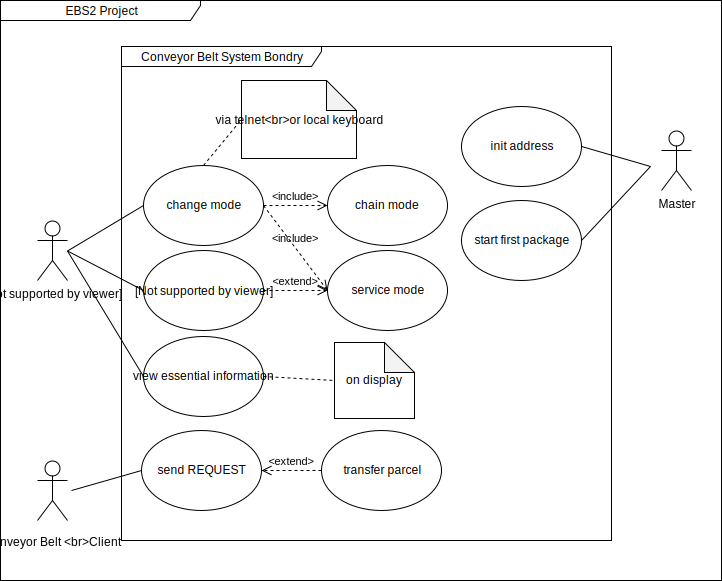
\includegraphics[width=\textwidth,height=\textheight,keepaspectratio]{useCaseDiagram/UseCaseDiagram.pdf}
	\caption[Use Case Diagram]{Use Case Diagram}
	\label{fig:UseCaseDiagram}
\end{figure}

\section{Sequence Diagram}
\label{chap:Sequence_Diagram}

\begin{figure}[H]
	\centering
	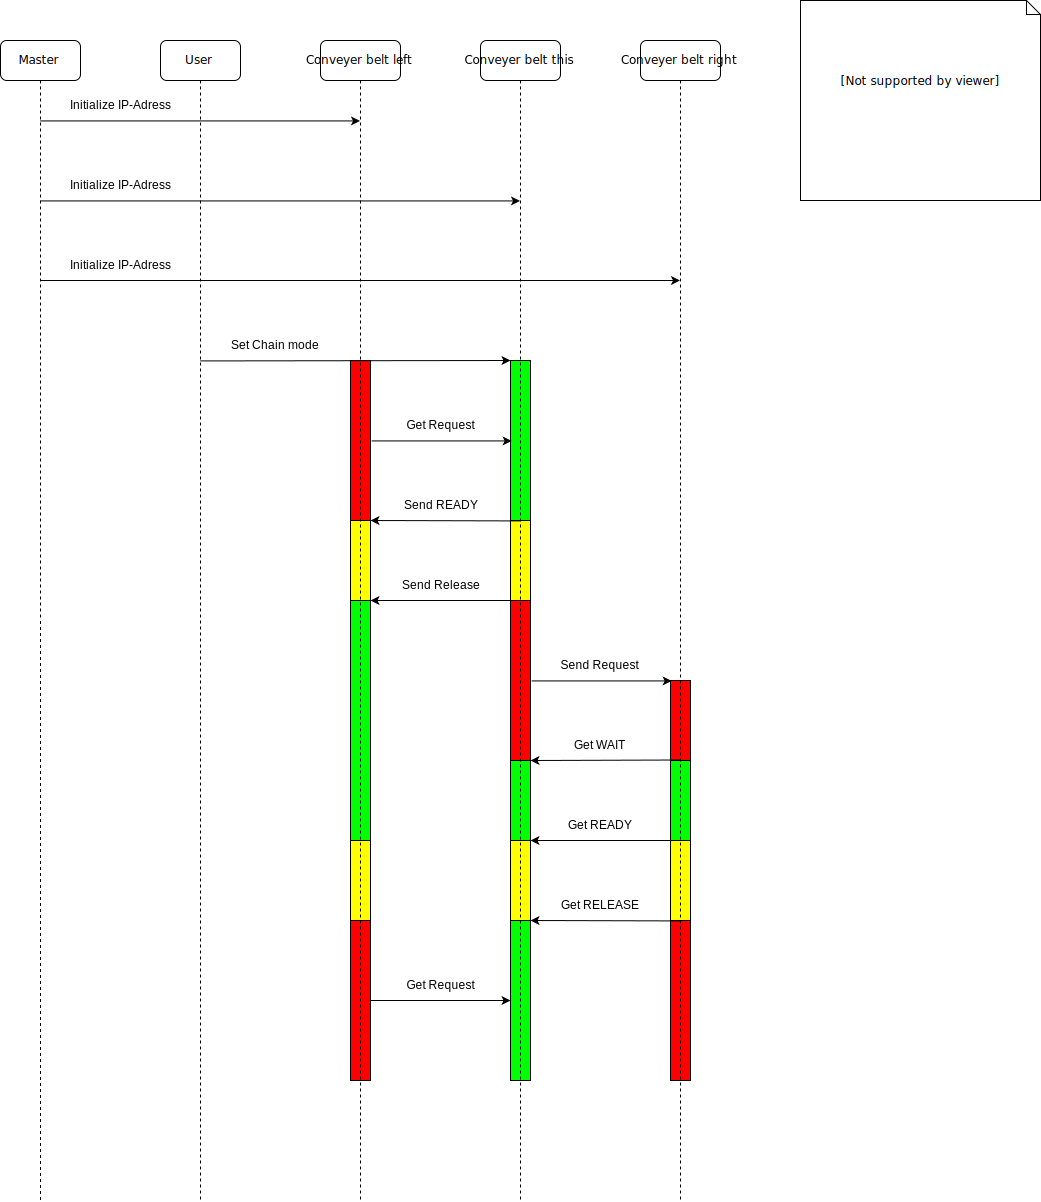
\includegraphics[width=\textwidth,height=\textheight,keepaspectratio]{sequenceDiagram/SequenceDiagram.pdf}
	\caption[Sequence Diagram]{Sequence Diagram}
	\label{fig:SequenceDiagram}
\end{figure}

\newpage

\section{Activity Diagram}
\label{chap:Activity_Diagram}

\begin{figure}[H]
	\centering
	\includegraphics[width=\textwidth,height=\textheight,keepaspectratio]{activityDiagram/activitychartIdleState.pdf}
	\caption[Activity Diagram Idle]{Activity Diagram Idle}
	\label{fig:ActivityDiagramIdle}
\end{figure}

\begin{figure}[H]
	\centering
	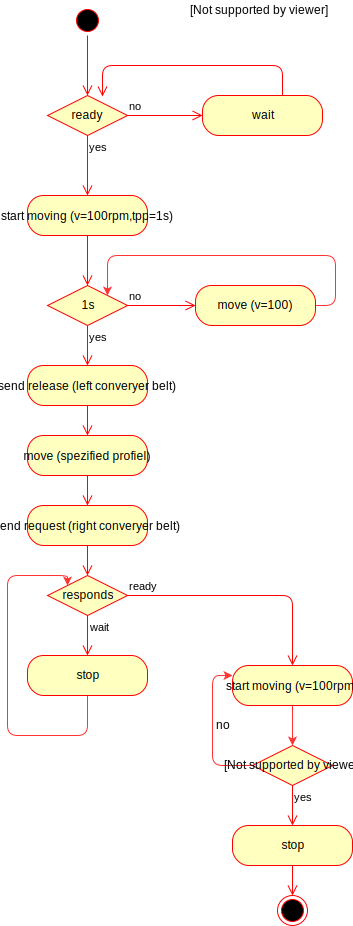
\includegraphics[width=\textwidth,height=\textheight,keepaspectratio]{activityDiagram/activitychartMovingState.pdf}
	\caption[Activity Diagram Moving]{Activity Diagram Moving}
	\label{fig:ActivityDiagramMoving}
\end{figure}

\begin{figure}[H]
	\centering
	\includegraphics[width=\textwidth,height=\textheight,keepaspectratio]{activityDiagram/activitychartServiceMode.pdf}
	\caption[Activity Diagram Service]{Activity Diagram Service}
	\label{fig:ActivityDiagramService}
\end{figure}

\chapter{Design}

\section{Class Diagram}
\label{chap:Class_Diagram}

In the following class diagram, the classes that are marked with a blue header are passive whereas the classes with the orange header are active and can actually make decisions themselves. The classes with the white header are interfaces. 

\begin{figure}[H]
	\centering
	\includegraphics[width=\textwidth,height=\textheight,keepaspectratio]{classDiagram/ClassDiagram.pdf}
	\caption[Class Diagram]{Class Diagram}
	\label{fig:ClassDiagram}
\end{figure}

\section{State Diagram}
\label{chap:State_Diagram}

The software is designed as three hierarchical state machines. The top-level diagram switches between the operation modes chain and service, which is shown in the first diagram. The following two diagrams show the lower level state machines. 

\begin{figure}[H]
	\centering
	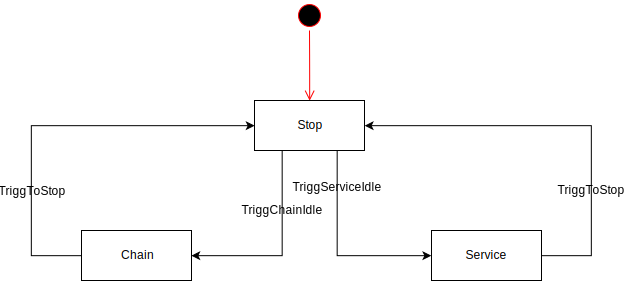
\includegraphics[width=\textwidth,height=\textheight,keepaspectratio]{stateDiagram/StateMachineMode.pdf}
	\caption[State Machine Mode]{State Machine Mode}
	\label{fig:StateMachineMode}
\end{figure}
\newpage

\begin{figure}[H]
	\centering
	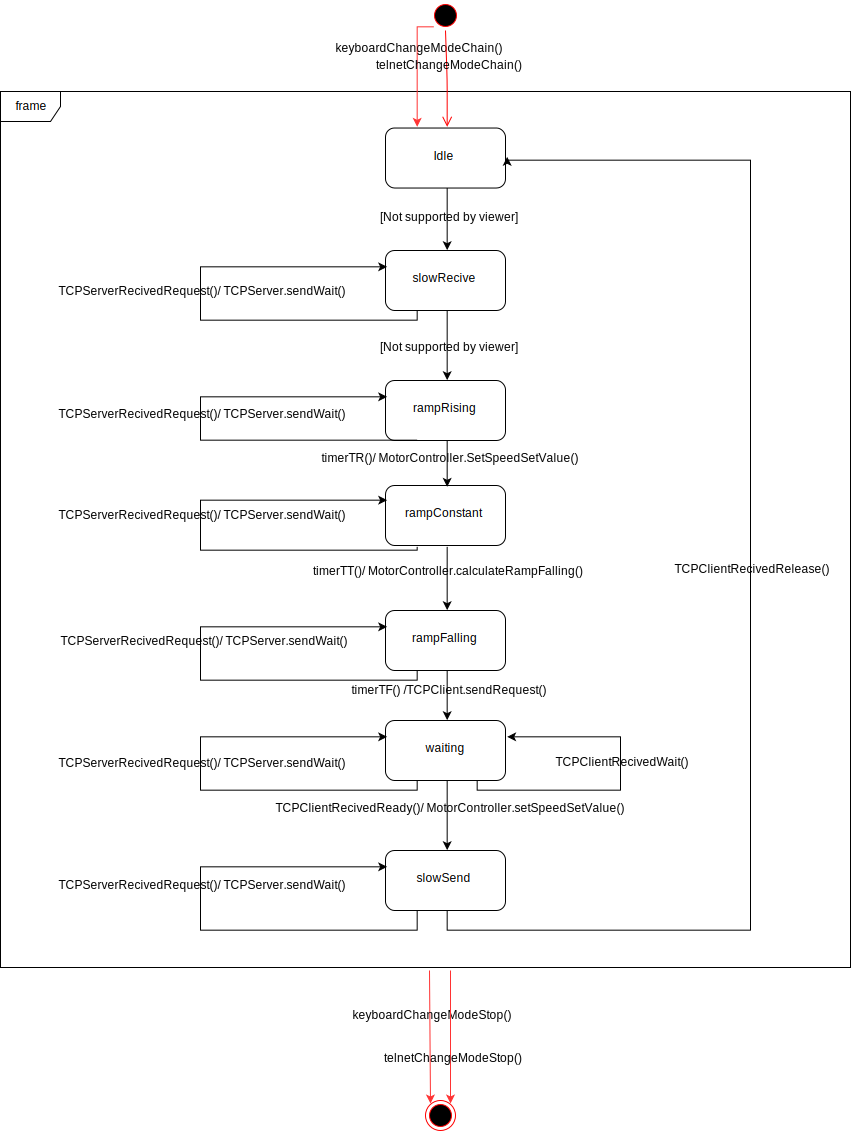
\includegraphics[width=\textwidth,height=\textheight,keepaspectratio]{stateDiagram/StateMachineChain.pdf}
	\caption[State Machine Chain]{State Machine Chain}
	\label{fig:StateMachineChain}
\end{figure}


\begin{figure}[H]
	\centering
	\includegraphics[width=\textwidth,height=\textheight,keepaspectratio]{stateDiagram/StateMachineService.pdf}
	\caption[State Machine Service]{State Machine Service}
	\label{fig:StateMachineService}
\end{figure}
 
\chapter{Summary}
\label{chap:Summary}


%\bibliographystyle{plain}
%\bibliography{Literatur}

\chapter*{Appendix A: Assignment}  % evtl. ersetzen mit \chapter*{Anhang}
\label{chap:AppendixAAssignment}
\addcontentsline{toc}{chapter}{Appendix A: Assignment}   % evtl. ersetzen mit \addcontentsline{toc}{chapter}{Anhang}
\includepdf[pages=-]{Assignment/_MEM2-ES_Project.pdf}


\chapter*{Appendix B: Requirements}  % evtl. ersetzen mit \chapter*{Anhang}
\label{chap:AppendixBRequirements}
\addcontentsline{toc}{chapter}{Appendix B: Requirements}   % evtl. ersetzen mit \addcontentsline{toc}{chapter}{Anhang}
\includepdf[pages=-]{Requirements/Requirements-Embeddes-Systems-Project.pdf}



\end{document}
